\documentclass[journal]{IEEEtran}

\usepackage{amsmath,amssymb}
\usepackage{booktabs}
\usepackage{cite}
\usepackage{graphicx}
\usepackage{multirow}

\newcommand{\method}{TurboADMM-NL}
\newcommand{\oldmethod}{TurboADMM}
\newcommand{\R}{\mathbb{R}}
\newcommand{\norm}[1]{\left\lVert #1\right\rVert}

% Generated by paper/ral/generate_results_macros.py; do not edit.
% paired_wall_aggregate_validation.csv sha256=d1218ddd8b17b0fef3b5f7af2381de3b948b93d67e2c3fb9ef8a0b59ed66238d
% full_vs_inner_aggregate_modern.csv sha256=9b4d267580e159d3ba984dde7baf40322ebd0b4ca4ea43b066c93b77b287b411
% full_vs_qp_continuation_aggregate_modern.csv sha256=d0b6287cf85853a1864eb747a5e7c31cf6b9a61ee531e175e6d0c9eea7d65514
% paired_statistics.csv sha256=5134b50903ca36eb14fa49b5258389f6d2395b66ae21f9f4153411568566fc94
% summary.csv sha256=712055a4c525c027a34e3131732dcc7648d70f7fbc2977aca6194a36e43f7fdd
\newcommand{\EvidenceStage}{development}
\newcommand{\PrimaryCases}{240}
\newcommand{\PrimaryStrictConvergences}{180}
\newcommand{\PrimaryOSQPStrictConvergences}{19}
\newcommand{\PrimaryMaximumObjectiveGapPercent}{4.735}
\newcommand{\WallRatioNFour}{0.816}
\newcommand{\WallRatioNEight}{1.369}
\newcommand{\WallRatioNTwelve}{1.905}
\newcommand{\WallRatioNTwenty}{2.439}
\newcommand{\AblationCases}{240}
\newcommand{\InnerRuntimeReductionPercent}{32.1}
\newcommand{\QPContinuationRuntimeReductionPercent}{32.3}
\newcommand{\ContinuationQPReductionPercent}{38.7}
\newcommand{\CSDOCases}{32}
\newcommand{\TurboCSDOSuccesses}{30}
\newcommand{\CSDOSuccesses}{15}
\newcommand{\CSDOBothValid}{15}
\newcommand{\TurboOnlyValid}{15}
\newcommand{\CSDOOnlyValid}{0}
\newcommand{\CSDONeitherValid}{2}
\newcommand{\CSDOMcNemarP}{6.10\times10^{-5}}
\newcommand{\PBSFailureCases}{17}
\newcommand{\TurboPBSRecoveries}{15}
\newcommand{\TurboPBSRecoveryPercent}{88.2}
\newcommand{\CSDOWilsonLowPercent}{30.9}
\newcommand{\CSDOWilsonHighPercent}{63.6}
\newcommand{\TurboWilsonLowPercent}{79.9}
\newcommand{\TurboWilsonHighPercent}{98.3}
\newcommand{\TurboCSDOMedianWallSeconds}{8.58}
\newcommand{\CSDOMedianWallSeconds}{0.099}

\IfFileExists{deterministic_results.tex}{% Generated by paper/ral/generate_deterministic_results.py; do not edit.
% results.csv sha256=6444cfaa1559256967d014371d219bb9a63a39a5a53abe284b8046aa24ab314c
% execution_status.csv sha256=e7d582787fbb4f3f99734d44e159500d7a2a966ee455470e68124412d88e5ce7
% run_manifest.json sha256=85fa380a72f42f7c1bbc01ec60303553d209b1775aee037a4c0873745f2ca568
\newcommand{\DeterministicRuns}{60}
\newcommand{\DeterministicStrict}{60}
\newcommand{\DeterministicMaximumObjectiveGapPercent}{2.319}
\newcommand{\DeterministicMinimumPairClearance}{1.22\times10^{-7}}
\newcommand{\DeterministicMinimumObstacleClearance}{-1.43\times10^{-3}}
\newcommand{\DeterministicMaximumDynamicsDefect}{0}
\newcommand{\DeterministicMaximumTerminalError}{3.01\times10^{-1}}
% Each cell is valid runs/repetitions; median wall time [s] on valid runs.
\newcommand{\DeterministicTableRows}{%
Easy open (2/0) & 10/10; 0.68 & 10/10; 0.31 & 10/10; 0.87 \\
Easy blocker (2/1) & 10/10; 1.12 & 10/10; 1.07 & 10/10; 1.82 \\
Medium doorway (4/2) & 10/10; 3.65 & 10/10; 26.46 & 10/10; 19.16 \\
Heterog. doorway (4/2) & 10/10; 8.94 & 10/10; 116.48 & 10/10; 105.54 \\
Warehouse (8/8) & 10/10; 54.15 & 0/10; -- & 0/10; -- \\
Maze (8/16) & 10/10; 67.93 & 0/10; -- & 0/10; -- \\
}
}{}
\title{TurboADMM-NL: Nested Parametric Continuation for Nonlinear
Heterogeneous Multi-Agent Trajectory Optimization}

% Update the complete author list and affiliations before submission.
\author{Yucheng Chen}

\begin{document}
\maketitle

\begin{abstract}
Nonlinear multi-agent trajectory optimization repeatedly solves coupled
quadratic programs whose temporal dynamics, collision geometry, and active
constraints evolve gradually. General-purpose centralized solvers do not
exploit agent separability, while conventional distributed methods repeatedly
discard useful state at nonlinear relinearization boundaries. This letter
extends our prior linear-QP solver, TurboADMM, to \method, a shared-memory
sequential convex programming method for heterogeneous robot teams. The method
combines per-agent alternating-direction decomposition with four levels of
structure reuse: affine Riccati initialization, vector hotstarts within each
ADMM solve, matrix and working-set continuation across nonlinear
linearizations, and geometry-aware transport of pairwise consensus and dual
state. A merit line search, trust-region restoration, elastic feasibility
recovery, and an independent continuous validator prevent continuation from
weakening nonlinear safety. The same problem may contain unicycles, bicycles,
and reduced-order three-dimensional quadcopters and convex polygonal
obstacles. Frozen deterministic and Monte Carlo protocols compare against
centralized qpOASES and OSQP and isolate each continuation layer. A disjoint
CSDO-compatible evaluation further tests a complementary property: repairing
locally conflicted trajectories from a common PBS/Hybrid-A* front end while
retaining negotiable inter-agent boundaries.
\end{abstract}

\begin{IEEEkeywords}
Multi-robot systems, trajectory optimization, distributed optimization,
sequential convex programming, ADMM.
\end{IEEEkeywords}

\section{Introduction}
\label{sec:introduction}
Multi-robot planning couples long-horizon nonlinear dynamics to pairwise
collision avoidance. A centralized transcription exposes all decision
variables and pair constraints to one optimizer. This is robust at small
scale, but the joint QP grows with the team and ignores the per-agent temporal
structure. Distributed optimization exposes parallelism, yet its many local QP
solves can erase that benefit when each solve is initialized independently.
The challenge becomes sharper inside sequential convex programming (SCP): an
ADMM loop solves one convexification, after which changed Jacobians and
separating planes conventionally trigger another cold optimization.

Our prior work \oldmethod~\cite{Chen2026TurboADMM} addressed a single sequence
of linearly constrained multi-agent QPs. It combined agent-level ADMM,
Riccati-based primal-dual initialization, and qpOASES active-set hotstarts.
That architecture reduced local QP work substantially, but it did not address
nonlinear dynamics, heterogeneous state dimensions, static obstacles, changing
collision geometry, nonlinear globalization, or recovery from an infeasible
reference. Merely placing the previous solver inside an SCP loop would discard
the active-set and consensus structure exactly where the nonlinear solver
spends most of its work.

This letter introduces \method, a nonlinear extension that treats the nested
SCP--ADMM iteration as a two-dimensional parametric sequence. At fixed
linearization, only consensus-dependent QP vectors change. Across SCP
iterations, dynamics matrices and collision normals change gradually. We reuse
the appropriate state at both boundaries and reset it only when a measurable
compatibility test fails. The method is algorithmically distributed but runs
on one shared-memory machine; it is not a network-distributed control scheme.

The contributions are:
\begin{itemize}
    \item A structure-preserving SCP decomposition for teams with mixed
    nonlinear models, agent-specific dimensions and footprints, convex
    polygonal obstacles, and inter-knot collision checking.
    \item Nested parametric continuation that combines Riccati initialization,
    inner-ADMM vector hotstarts, cross-SCP matrix/working-set continuation, and
    geometry-aware transport of pairwise auxiliary and scaled-dual state.
    \item A strict nonlinear recovery mechanism combining exact rollout,
    merit globalization, cold reliable QP reconstruction, elastic slacks,
    trust-region contraction, and final fixed-penalty consensus polishing.
    \item A frozen evaluation protocol with six hand-designed cases, a
    24-cell Monte Carlo scaling matrix, centralized qpOASES and OSQP baselines,
    continuation ablations, and a disjoint paired CSDO recovery study.
\end{itemize}

The novelty is not ADMM, Riccati recursion, active-set hotstarting, or SCP in
isolation. It is their continuation-aware composition across both levels of a
nonlinear multi-agent solver, together with evidence that the added reuse
reduces work without relaxing feasibility or objective-quality gates.

\section{Related Work}
\label{sec:related}
Sparse first-order QP solvers such as OSQP~\cite{Stellato2020OSQP} are robust
general baselines, and parametric active-set solvers such as
qpOASES~\cite{Ferreau2014qpOASES} can exploit similarity between consecutive
QPs. Optimal-control solvers exploit block temporal structure, but a
monolithic multi-agent transcription still exposes growing coupling. Our
focus is orthogonal: retain separate per-agent optimal-control QPs and move the
coupling into low-dimensional consensus projections.

ADMM provides a standard mechanism for decomposing convex programs with
coupling constraints~\cite{Boyd2011ADMM}. Multi-agent variants range from
physically distributed control and DDP architectures~\cite{Saravanos2023DDP}
to centralized shared-memory decomposition. The latter is the relevant
comparison here: communication latency is absent, so performance depends on
local QP work, parallel scheduling, and the number of consensus rounds.
\oldmethod~\cite{Chen2026TurboADMM} showed that Riccati initialization and
parametric active-set hotstarts are complementary for linear multi-agent QPs.
\method extends that mechanism across nonlinear relinearizations rather than
claiming a new ADMM splitting.

Recent decentralized planners make different coupling choices. Robust
MADER~\cite{Kondo2023RobustMADER} optimizes against communicated trajectories
and explicitly protects asynchronous execution from communication delay.
Spatiotemporal-occupancy methods~\cite{Wu2024SOGM} embed shared trajectories
into local maps and construct independent safe corridors, while
MA-DV$^2$F~\cite{Ma2025MADV2F} generates dynamic velocity fields independently
for nonholonomic vehicles. These methods prioritize reactive or onboard
decentralized navigation. In contrast, \method is a batch optimizer on one
shared-memory machine: it retains negotiable pair constraints during every SCP
step, but does not claim communication-delay robustness or feedback-control
rates.

Sequential convex optimization is widely used to obtain locally optimal
collision-free trajectories~\cite{Schulman2013TrajOpt}. Its performance and
robustness depend on the reference homotopy, trust-region policy, and recovery
from temporarily infeasible convexifications. We preserve a nonlinear merit
test and independently validate every returned trajectory; a feasible
SCP-limit iterate is reported separately from strict convergence.

CSDO~\cite{Yang2024CSDO} combines centralized priority-based search (PBS) and
spatiotemporal Hybrid-A* with decentralized QP refinement. Its separating
planes and safe corridors are constants derived from the initial guess, so
each vehicle QP is independent. This makes refinement extremely fast when the
searched homotopy and assignment of avoidance responsibility are already
adequate. Our CSDO experiment keeps the same search front end but asks a
different question: can a coupled optimizer repair a locally conflicted root
by negotiating pairwise motion rather than accepting fixed mutual boundaries?
Runtime is therefore secondary in that comparison and is disclosed as a
non-advantage.

\section{Nonlinear Multi-Agent Problem}
\label{sec:problem}
Consider $N$ agents over horizon $H$. Agent $i$ has state
$x_{i,k}\in\R^{n_i}$, input $u_{i,k}\in\R^{m_i}$, discrete dynamics
$f_i$, and position output $h_i$. An embedding $E_i$ maps a two- or
three-dimensional position into the common workspace $\R^d$, where
$d=\max_i\dim h_i$. The dynamics and position maps are
\begin{align}
 x_{i,k+1} &= f_i(x_{i,k},u_{i,k}), \\
 p_{i,k} &= E_i h_i(x_{i,k}).
\end{align}
Each agent has radius $r_i$; ground footprints are discs and aerial footprints
are spheres. Polygonal obstacles are treated as vertical prisms when $d=3$.

With local stage and terminal costs $\ell_i$ and $\phi_i$, the joint problem is
\begin{subequations}\label{eq:nlp}
\begin{align}
 \min_{x,u}\quad & \sum_{i=1}^N\left[
 \phi_i(x_{i,H})+\sum_{k=0}^{H-1}\ell_i(x_{i,k},u_{i,k})\right] \\
 \mathrm{s.t.}\quad
 &x_{i,k+1}=f_i(x_{i,k},u_{i,k}), \\
 &(x_{i,k},u_{i,k})\in\mathcal X_{i,k}\times\mathcal U_{i,k}, \\
 &\norm{p_{i,k}-p_{j,k}}_2\ge r_i+r_j,\quad i<j, \\
 &\operatorname{dist}(p_{i,k},\mathcal O_q)\ge r_i,
\end{align}
\end{subequations}
together with masked terminal equalities or terminal tolerances. Collision
constraints are enforced both at knots and interpolated substeps. Problem
\eqref{eq:nlp} is nonconvex because of the dynamics and reverse-convex
separation constraints.

The implementation supports the model set in Table~\ref{tab:models}. A single
problem may mix all three. The quadcopter is deliberately reduced order; a
full rigid-body torque model is outside the present claim.

\begin{table}[t]
\caption{Implemented heterogeneous agent models.}
\label{tab:models}
\centering
\begin{tabular}{lccc}
\toprule
Model & $n_i$ & $m_i$ & Position \\
\midrule
Unicycle & 4 & 2 & $(p_x,p_y)$ \\
Bicycle & 5 & 2 & $(p_x,p_y)$ \\
Reduced quadcopter & 9 & 4 & $(p_x,p_y,p_z)$ \\
\bottomrule
\end{tabular}
\end{table}

\section{TurboADMM-NL}
\label{sec:method}

\subsection{Structure-Preserving Convexification}
At SCP iteration $s$, let $(\bar x^s,\bar u^s)$ be the nominal trajectory and
use increments $(\delta x,\delta u)$. Linearized dynamics are
\begin{equation}
 \delta x_{i,k+1}=A^s_{i,k}\delta x_{i,k}
 +B^s_{i,k}\delta u_{i,k}+d^s_{i,k},
\label{eq:linear-dynamics}
\end{equation}
where $A^s_{i,k}$ and $B^s_{i,k}$ are analytic Jacobians and $d^s_{i,k}$ is
the affine defect. For pair $(i,j)$, define nominal displacement
$\bar q^s_{ij,k}=\bar p^s_{i,k}-\bar p^s_{j,k}$ and unit normal
$n^s_{ij,k}=\bar q^s_{ij,k}/\norm{\bar q^s_{ij,k}}_2$. The supporting
half-space is
\begin{equation}
 (n^s_{ij,k})^T\left(J^s_{i,k}\delta x_{i,k}
 -J^s_{j,k}\delta x_{j,k}\right)
 \ge r_i+r_j-(n^s_{ij,k})^T\bar q^s_{ij,k}.
\label{eq:pair-halfspace}
\end{equation}
Convex polygon constraints use supporting planes on clearance-inflated
boundaries. A proximity margin screens inactive pairs and obstacles in the
constant-density experiments; the nonlinear merit and independent validator
still evaluate every pair and obstacle.

\subsection{Agent-Level ADMM}
Collect agent $i$'s increments in $w_i$. The convexified objective and local
constraints give
\begin{equation}
 \min_{w_i\in\mathcal W_i^s}\frac{1}{2}w_i^T H_i^s w_i
 +(g_i^s)^T w_i,
\end{equation}
where $\mathcal W_i^s$ contains \eqref{eq:linear-dynamics}, bounds, terminal
rows, trust-region rows, and static-obstacle half-spaces. For each active
pair-stage incidence $e$, a selector $P_{i,e}^s$ exposes the local position
used by \eqref{eq:pair-halfspace}. Introducing auxiliary positions $z_e$ and
scaled duals $y_{i,e}$ yields the local ADMM update
\begin{equation}
 \begin{aligned}
 w_i^{r+1}=\arg\min_{w_i\in\mathcal W_i^s}\;&
 \frac{1}{2}w_i^T H_i^s w_i+(g_i^s)^T w_i\\
 &+\frac{\rho}{2}\sum_{e\in\mathcal E_i^s}
 \norm{P_{i,e}^s w_i-z_{i,e}^r+y_{i,e}^r}_2^2.
 \end{aligned}
\label{eq:local-qp}
\end{equation}
All local QPs are independent and are solved in parallel. The coordinator
projects each two-agent auxiliary block onto its collision half-space and then
updates the scaled duals. Thus no centralized coupling QP is solved.

\subsection{Nested Parametric Continuation}
The architecture reuses structure at four distinct boundaries.
\begin{enumerate}
    \item \emph{Riccati initialization.} At the first local solve, an affine,
    stage-varying LQR recursion produces a dynamics-feasible primal trajectory
    and equality multipliers in $O(H)$ stage operations. Inequality multipliers
    begin at zero.
    \item \emph{Inner vector hotstart.} Within one SCP linearization, the
    Hessian and constraint matrix of \eqref{eq:local-qp} are fixed while the
    consensus-dependent gradient and bounds vary. qpOASES reuses the previous
    primal-dual point and active set.
    \item \emph{Cross-SCP matrix hotstart.} When $A^s$, $B^s$, obstacle rows,
    or collision rows change, qpOASES receives the new matrices while retaining
    the compatible working set and local solution.
    \item \emph{Geometry-aware consensus transport.} A pair-stage state is
    transported only if
    $(n^{s-1}_{ij,k})^Tn^s_{ij,k}\ge\gamma$. Its auxiliary positions are
    projected onto the new half-space and only the dual component aligned with
    $n^s_{ij,k}$ is retained. Incompatible states are reset from the nominal
    trajectory.
\end{enumerate}
These mechanisms define four controlled ablations: \emph{cold}, \emph{inner},
\emph{QP continuation}, and \emph{full}. All variants share the same model,
linearization, cost, initialization, penalty, trust region, and tolerances.
Continuation changes only the initialization of the local active-set and ADMM
iterations. Conditioned on convergence of a convexified subproblem, every
variant therefore satisfies the same primal feasibility and ADMM fixed-point
conditions; transported pair state neither changes the objective nor removes a
constraint. Projection of compatible auxiliaries and reset of incompatible
state preserve this invariant across relinearizations. Nonlinear feasibility is
then enforced separately by globalization and the independent validator.

\subsection{Globalization and Feasibility Recovery}
A nonlinear merit line search accepts an SCP candidate only when the true
rollout improves the frozen merit. Full-state references are projected through
the exact nonlinear dynamics whenever this restores dynamics without violating
physical safety. If a convex subproblem fails, the solver rebuilds it cold
with reliable active-set settings. A second fallback introduces nonnegative
elastic slacks on temporarily infeasible obstacle, corridor, and terminal
rows, penalized by a fixed exact-penalty weight. Rejected steps roll back to the
last accepted nonlinear iterate and contract the control trust region.

After the ordinary convergence predicate first holds, a fixed-$\rho$ phase
polishes consensus with zero relative residual tolerance. Restoration slacks
must vanish, the QP direction must meet the unchanged SCP step tolerance, and
the nonlinear trajectory must satisfy pair, obstacle, dynamics, and terminal
tests before strict convergence is declared.

\subsection{Structural Scaling}
Let $q_i=O(H(n_i+m_i))$ be one local QP dimension, $\Delta$ the maximum active
interaction degree, and $P$ the number of worker threads. One ADMM round costs
approximately
\begin{equation}
 O\!\left(\frac{1}{P}\sum_i C_{\mathrm{QP}}(q_i)
 +H|\mathcal E^s|d\right),
\end{equation}
whereas a centralized solver processes dimension $\sum_iq_i$ and all coupling
rows simultaneously. \method\ does not claim a universal asymptotic bound for
active-set work. Its intended regime is spatially local interaction, where
$\Delta$ and local QP dimensions remain bounded while the centralized problem
continues to grow. The experiments report active degree, QP dimensions, QP
solves, working-set recalculations, solver time, process wall time, and peak
memory rather than inferring scalability from runtime alone.

\section{Experimental Protocol}
\label{sec:protocol}
All publication runs use the same WSL Release binary and independent nonlinear
validator. Collision and obstacle clearance are sampled at 20 substeps per
interval. A run succeeds only if solver execution finishes under the frozen
cap and the validator accepts pair clearance, obstacle clearance, nonlinear
dynamics, and terminal constraints. Strict SCP convergence is reported
separately and is required for every Turbo deterministic and development-gate
case. Run manifests hash the executable, runner, scenario inventory, method
order, and OpenMP policy.

\subsection{Comparisons and Ablations}
The internal comparisons are centralized qpOASES and official OSQP applied to
the identical SCP QP, plus the cold, inner, QP-continuation, and full
distributed variants. Deterministic timings use ten fresh processes with
interleaved method order. Monte Carlo uses paired seeds and reports medians,
quartiles, Wilson success intervals, exact paired sign tests for crossover,
and objective gaps on jointly valid outputs. All six variants run on
development; the untouched final split repeats only full, centralized OSQP,
and centralized qpOASES because the ablation is frozen on 240 development cases.

\subsection{Scenario Sets}
The six headline deterministic cases progress from a two-unicycle open
crossing to a single blocker, a four-agent doorway, a heterogeneous doorway,
an eight-agent warehouse, and an eight-agent maze. A heterogeneous open case
remains a regression-only overhead control and is not used as headline
performance evidence.

The submission-primary Monte Carlo grid contains
$N\in\{4,8,12,20\}$, obstacle counts $M\in\{0,N,2N\}$, homogeneous
unicycles and balanced heterogeneous teams, and ten development or thirty
untouched final seeds per cell. Constant-density local exchanges provide an
analytic feasibility witness and are designed to keep active interaction
degree bounded. This gives 240 development and 720 final scenarios.

For CSDO, both branches use the untouched, deterministically seeded
PBS/Hybrid-A* front end. On search success, CSDO's pre-DSQP initial guess is
passed directly to \method. A clean-source exporter repeats the same seeded
search, verifies schedule equality to $10^{-9}$, and reconstructs the static
obstacle corridors before either optimization branch is run.
Original CSDO then constructs fixed inter-agent separating planes and solves
independent vehicle QPs; \method\ instead retains negotiable pair coupling. If
PBS fails, the exporter preserves a conflicted root when PBS exposes one. If
PBS exposes no root, it runs the same Hybrid-A* search independently for each
vehicle, producing individually feasible but mutually conflicted paths.
Either failure artifact and its reconstructed static corridors become
\method's input, while original CSDO reports search failure. \method\ may
widen only the temporal indexing of the reconstructed static corridor under
the frozen recovery rule. Every source, executable, schedule, and corridor
artifact is hashed. Development uses 24 passing-bay
instances; evaluation uses a disjoint 32-case grid varying bay length, arrival
offset, and priority order.

\section{Results}
\label{sec:results}
% The primary-final tables are intentionally not populated until the solver is
% frozen and the untouched 720-case split is executed once.

\ifdefined\DeterministicTableRows
\subsection{Deterministic Stress Tests}
\begin{table*}[t]
\caption{Frozen deterministic stress tests. Each entry is valid runs/10;
median WSL process wall time in seconds among valid runs. Parentheses in the
scenario column give agents/obstacles.}
\label{tab:deterministic}
\centering
\scriptsize
\begin{tabular}{lccc}
\toprule
Scenario ($N/M$) & \method & OSQP & qpOASES \\
\midrule
\DeterministicTableRows
\bottomrule
\end{tabular}
\end{table*}
\method{} validates and strictly converges on
\DeterministicStrict/\DeterministicRuns{} runs. Its maximum absolute objective
gap on jointly valid OSQP outputs is
\DeterministicMaximumObjectiveGapPercent\%. The maximum terminal error and
dynamics defect are $\DeterministicMaximumTerminalError$ and
$\DeterministicMaximumDynamicsDefect$; minimum sampled pair and obstacle
clearances are $\DeterministicMinimumPairClearance$ and
$\DeterministicMinimumObstacleClearance$, within the fixed $10^{-2}$
collision tolerance.
\fi

\subsection{Development Gates}
The frozen development evidence establishes the intended crossover but is not
substituted for the untouched final matrix. On \PrimaryCases\ paired scenarios, both
\method\ and centralized OSQP return independently valid, strictly converged
trajectories. The
median OSQP/\method\ process-wall ratios are $\WallRatioNFour$,
$\WallRatioNEight$, $\WallRatioNTwelve$, and $\WallRatioNTwenty$ for
$N=4,8,12,20$, respectively. The crossover occurs near $N=8$ and is
statistically significant at $N=12$ ($p=\WallSignPNtwelve$) and $N=20$
($p=\WallSignPNtwenty$). At $N=20$, centralized OSQP uses
$\MemoryRatioNTwenty\times$ the median peak memory. The maximum absolute
objective gap is \PrimaryMaximumObjectiveGapPercent\%, below the predeclared
5\% gate.

\begin{figure}[t]
\centering
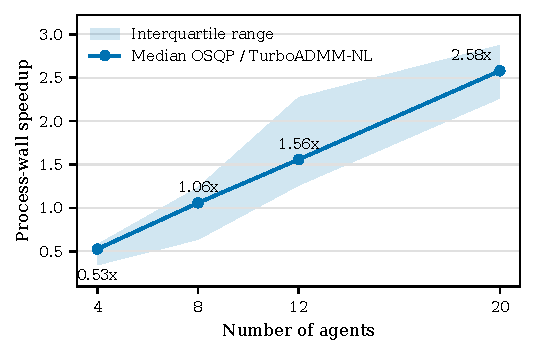
\includegraphics[width=\columnwidth]{figures/scaling-crossover.pdf}
\caption{\EvidenceStageLabel{} scaling on \PrimaryCasesPerScale{} paired
cases per team size. Values above
one favor \method; shading is the interquartile range.}
\label{fig:scaling}
\end{figure}

\ifdefined\PrimaryQpOASESSuccessNFour
\begin{table*}[t]
\caption{Untouched final matrix. Entries are valid trajectories/180 and
median WSL process wall time in seconds among valid runs.}
\label{tab:primary-final}
\centering
\scriptsize
\begin{tabular}{c@{\quad}cc@{\quad}cc@{\quad}cc}
\toprule
 & \multicolumn{2}{c}{\method} & \multicolumn{2}{c}{OSQP}
 & \multicolumn{2}{c}{qpOASES} \\
$N$ & Valid & Wall & Valid & Wall & Valid & Wall \\
\midrule
4 & \PrimaryTurboSuccessNFour & \PrimaryTurboWallNFour
  & \PrimaryOSQPSuccessNFour & \PrimaryOSQPWallNFour
  & \PrimaryQpOASESSuccessNFour & \PrimaryQpOASESWallNFour \\
8 & \PrimaryTurboSuccessNEight & \PrimaryTurboWallNEight
  & \PrimaryOSQPSuccessNEight & \PrimaryOSQPWallNEight
  & \PrimaryQpOASESSuccessNEight & \PrimaryQpOASESWallNEight \\
12 & \PrimaryTurboSuccessNTwelve & \PrimaryTurboWallNTwelve
  & \PrimaryOSQPSuccessNTwelve & \PrimaryOSQPWallNTwelve
  & \PrimaryQpOASESSuccessNTwelve & \PrimaryQpOASESWallNTwelve \\
20 & \PrimaryTurboSuccessNTwenty & \PrimaryTurboWallNTwenty
  & \PrimaryOSQPSuccessNTwenty & \PrimaryOSQPWallNTwenty
  & \PrimaryQpOASESSuccessNTwenty & \PrimaryQpOASESWallNTwenty \\
\bottomrule
\end{tabular}
\end{table*}
\fi

The continuation ablation contains \AblationCases\ common scenarios for each
distributed variant. Matrix/working-set continuation reduces median runtime by
\MatrixContinuationRuntimeReductionPercent\% relative to inner vector
hotstarts alone. Adding geometry-aware pair-state transport yields a further
\PairTransportRuntimeReductionPercent\% overall and
\PairTransportRuntimeReductionNTwentyPercent\% at $N=20$, while reducing the
median number of local QP solves by \PairTransportQPReductionPercent\%.
Together, the full cross-SCP continuation stack reduces median runtime by
\FullContinuationRuntimeReductionPercent\%. Every variant validates and
strictly converges on all \AblationCases\ cases.

\begin{figure*}[t]
\centering
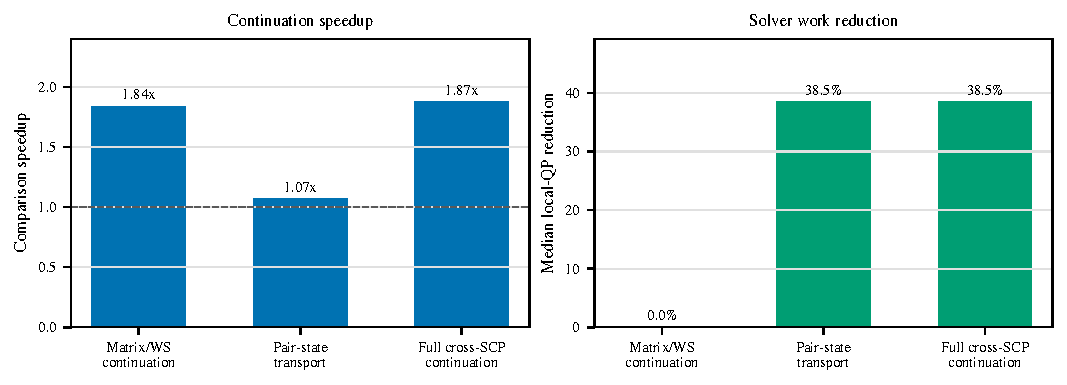
\includegraphics[width=0.78\textwidth]{figures/continuation-ablation.pdf}\\[-0.5ex]
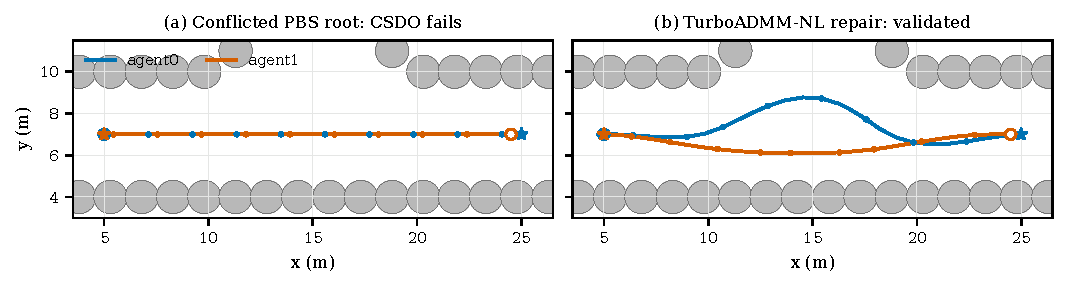
\includegraphics[width=0.82\textwidth]{figures/csdo-repair.pdf}
\caption{Top: causal continuation ablation on the development matrix,
isolating matrix/working-set reuse, pair-state transport, and their combined
cross-SCP effect. Bottom: a representative frozen CSDO-compatible recovery.
PBS terminates with mutually conflicted centerline trajectories (left);
starting from that exact artifact and its static corridors, \method\
negotiates which vehicle enters the bay and returns an independently validated
plan (right). Circles are CSDO map obstacles and dots are equal-time samples.}
\label{fig:ablation-recovery}
\end{figure*}

\subsection{CSDO-Compatible Recovery}

Table~\ref{tab:csdo} reports every case in the disjoint evaluation grid.
\method\ validates \TurboCSDOSuccesses\ of \CSDOCases\ cases, versus
\CSDOSuccesses\ of \CSDOCases\ for original CSDO. The paired outcomes contain
\CSDOBothValid\ shared successes, \TurboOnlyValid\ \method-only successes,
\CSDOOnlyValid\ CSDO-only successes, and \CSDONeitherValid\ joint failures.
The exact two-sided McNemar test is $p=\CSDOMcNemarP$. Of \PBSFailureCases\
cases where CSDO's PBS search fails, \method\ repairs \TurboPBSRecoveries\
(\TurboPBSRecoveryPercent\%), while CSDO repairs none.
These comprise \PBSRootFailureCases\ retained-root cases and
\IndependentPathFailureCases\ cases initialized from mutually conflicted
single-agent Hybrid-A* paths. Every success is checked by the same continuous
validator.

\begin{table}[t]
\caption{Frozen paired CSDO evaluation (\CSDOCases\ cases).}
\label{tab:csdo}
\centering
\begin{tabular}{lcc}
\toprule
Metric & CSDO & \method \\
\midrule
Independently valid & \CSDOSuccesses/\CSDOCases & \TurboCSDOSuccesses/\CSDOCases \\
PBS-failure recovery & 0/\PBSFailureCases & \TurboPBSRecoveries/\PBSFailureCases \\
Method-only successes & \CSDOOnlyValid & \TurboOnlyValid \\
95\% Wilson interval & [\CSDOWilsonLowPercent,\CSDOWilsonHighPercent]\% &
[\TurboWilsonLowPercent,\TurboWilsonHighPercent]\% \\
\bottomrule
\end{tabular}
\end{table}

The recorded times do not have identical scope and therefore are not used for
a runtime comparison. CSDO's searched separating planes eliminate all
optimization coupling, whereas \method\ retains and negotiates pair
constraints. This experiment isolates the resulting recovery capability, not
speed. On shared successes, median path length differs by only
\SharedPathReductionPercent\%, so we also make no broad reduced-conservatism
claim from this suite.

\subsection{Required Final Evidence}
Before submission, the frozen solver must pass: (i) all six headline
deterministic tests and the retained heterogeneous-open overhead control,
(ii) all 240 development strict-convergence rows with
no objective gap above 5\%, (iii) the continuation novelty gate without loss
of success, and (iv) one untouched 720-case final run. The final paper tables
will report success, strict convergence, objective quality, wall and solver
time, peak memory, SCP/ADMM work, active degree, and centralized/local QP
dimensions. No parameter may change after the final split is inspected.

\section{Limitations}
\label{sec:limitations}
\method\ is a local nonlinear optimizer and does not replace global homotopy
search. Its deterministic polygon bypass is suitable for the tested convex
obstacles; complicated maps still benefit from a feasible reference or a
search front end. The quadcopter model omits full rigid-body angular dynamics.
Shared-memory decomposition does not address communication delay or packet
loss. Finally, continuation can reduce repeated QP work but does not guarantee
fewer SCP or ADMM iterations on every small problem; the claimed advantage is
the bounded-degree medium-to-large regime and the ability to negotiate
coupling that fixed-corridor refiners remove.

\section{Conclusion}
\label{sec:conclusion}
This letter extends \oldmethod\ from structured linear multi-agent QPs to
nonlinear heterogeneous trajectory optimization. The key mechanism is nested
parametric continuation: temporal Riccati structure, active-set information,
and geometry-aligned consensus state are reused at the iteration boundary where
each is valid. Strict globalization and independent validation preserve safety.
The frozen experiments are designed to test two complementary claims rather
than one universal speed claim: structural crossover against centralized QP
solvers and recovery of locally conflicted search trajectories that fixed
separating planes cannot negotiate.

\bibliographystyle{IEEEtran}
\bibliography{references}
\end{document}
